
Laskeutuminen on se hypyn vaihe, jossa sattuu eniten loukkaantumisia. Seuraavissa kappaleissa on esimerkkejä erilaisista laskeutumisvirheistä. Yksi virhe ei välttämättä aiheuta loukkaantumista, mutta usean virheen yhdistelmän seurauksena voi olla loukkaantuminen. Hypättäessä suuremmalla siipikuormalla ja suorituskykyisemmällä varjolla virheiden merkitys korostuu. Jos ajattelet vaihtaa varjosi aiempaa suorituskykyisempään, karsi ensin virheet laskeutumisistasi ja harjoittele erilaisia laskeutumistekniikoita. 

\section{ Vauhdin puute }
\label{laskeutumisvirheet-vauhdin-puute}


Loppuveto tehoaa sitä paremmin, mitä suurempi vauhti on. Vauhdin tappaminen finaalissa turhalla jarrutuksella tai peräkkäisillä ohjausliikkeillä heiluttamalla vähentää loppuvedon tehokkuutta. Finaaliin kääntyessään jotkut tekevät heilahtavan käännöksen ohjauslenkeistä suhteellisen korkealla, jolloin varjo käännöksen jälkeen fleeraa kuin itsestään ja alkaa sen jälkeen taas kerätä nopeutta. Jos oikea fleeri pitää suorittaa sillä hetkellä, kun varjo vasta kerää vauhtia, tulee siitä varsin tehoton. Pidä täysiliito koko finaalin ajan ja vältä turhia peräkkäisiä ohjausliikkeitä ja jarrutuksia. 

\section{ Pumppaaminen }
\label{laskeutumisvirheet-pumppaaminen}


Liitovarjojen tullessa markkinoille opetettiin varjosta ottamaan vauhti pois pumppaamalla. Turha pumppaaminen tappaa vauhdin ja heikentää loppuvedon vaikutusta. Pidä täysliito koko finaalin ajan ja vältä turhaa pumppaamista loppuvedossa. Eivät lentokoneetkaan laskeudu laskulaippoja sisään ja ulos liikuttaen. 

\section{ Löysä loppuveto }
\label{laskeutumisvirheet-loysa-loppuveto}


Löysä loppuveto on yleisin virhe laskeuduttaessa. Kun loppuveto aloitetaan liian korkealla ja tehdään hitaasti alas asti, ei varjon liikesuunta muutu maanpinnan suuntaiseksi, koska hyppääjä ei heilahda eteenpäin kuvun alla. Tuloksena on kova lasku. 

\section{ Liian lyhyt loppuveto tai ei loppuvetoa }
\label{laskeutumisvirheet-liian-lyhyt-loppuveto-tai-ei-loppuvetoa}


Liian lyhyt loppuveto tai koko loppuvedon tekemättä jättäminen ei käännä kuvun liikesuuntaa vaakalentoon ja seurauksena on kova lasku. Loppuvedon unohtaminen voi johtua mm. keskittymisestä muuhun liikenteeseen tai yllättävästä tilanteesta finaalissa. Myös tarkkuuskilpailuissa keskitytään laskeutumaan mahdollisimman lähelle maalia ja loppuveto unohtuu. 

\section{ Epätasainen loppuveto }
\label{laskeutumisvirheet-epatasainen-loppuveto}


Epätasainen loppuveto kääntää varjon suuntaa. Tätä seuraa yleensä suojautumisansa, jolloin kädellä vaistomaisesti suojataan liikesuunnan sivuttaismuutosta. Yleensä oikeakätinen vetää oikealla kädellä enemmän ja päinvastoin. 


\begin{Figure}\centering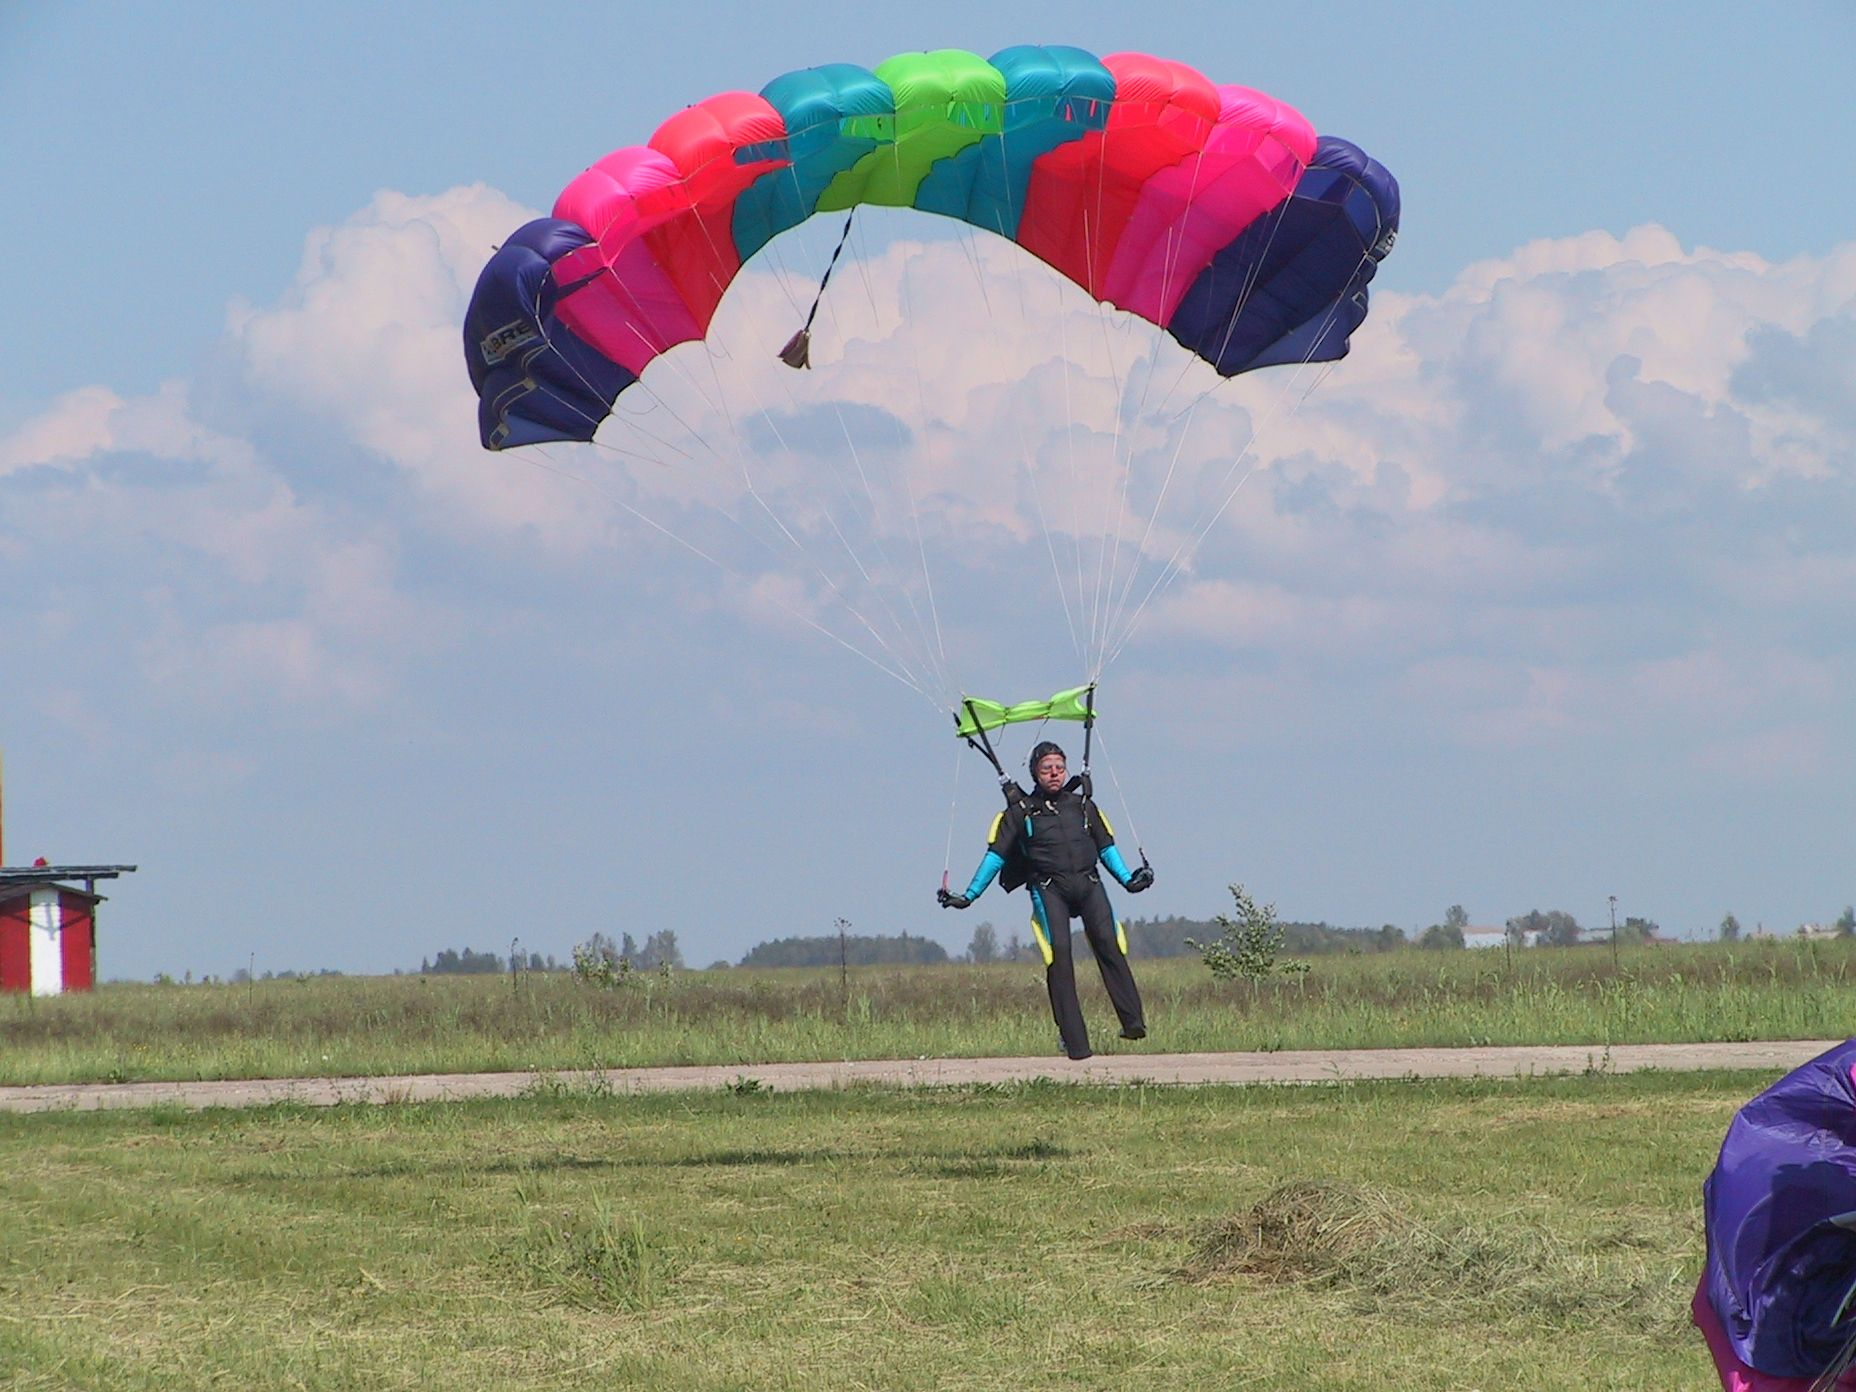
\includegraphics[width=0.99\textwidth]{Loppuveto_epatasainen.jpeg}\captionof{figure}{Epätasainen loppuveto oikea käsi alempana, varjo kaatuu oikealle.}\end{Figure}  \begin{Figure}\centering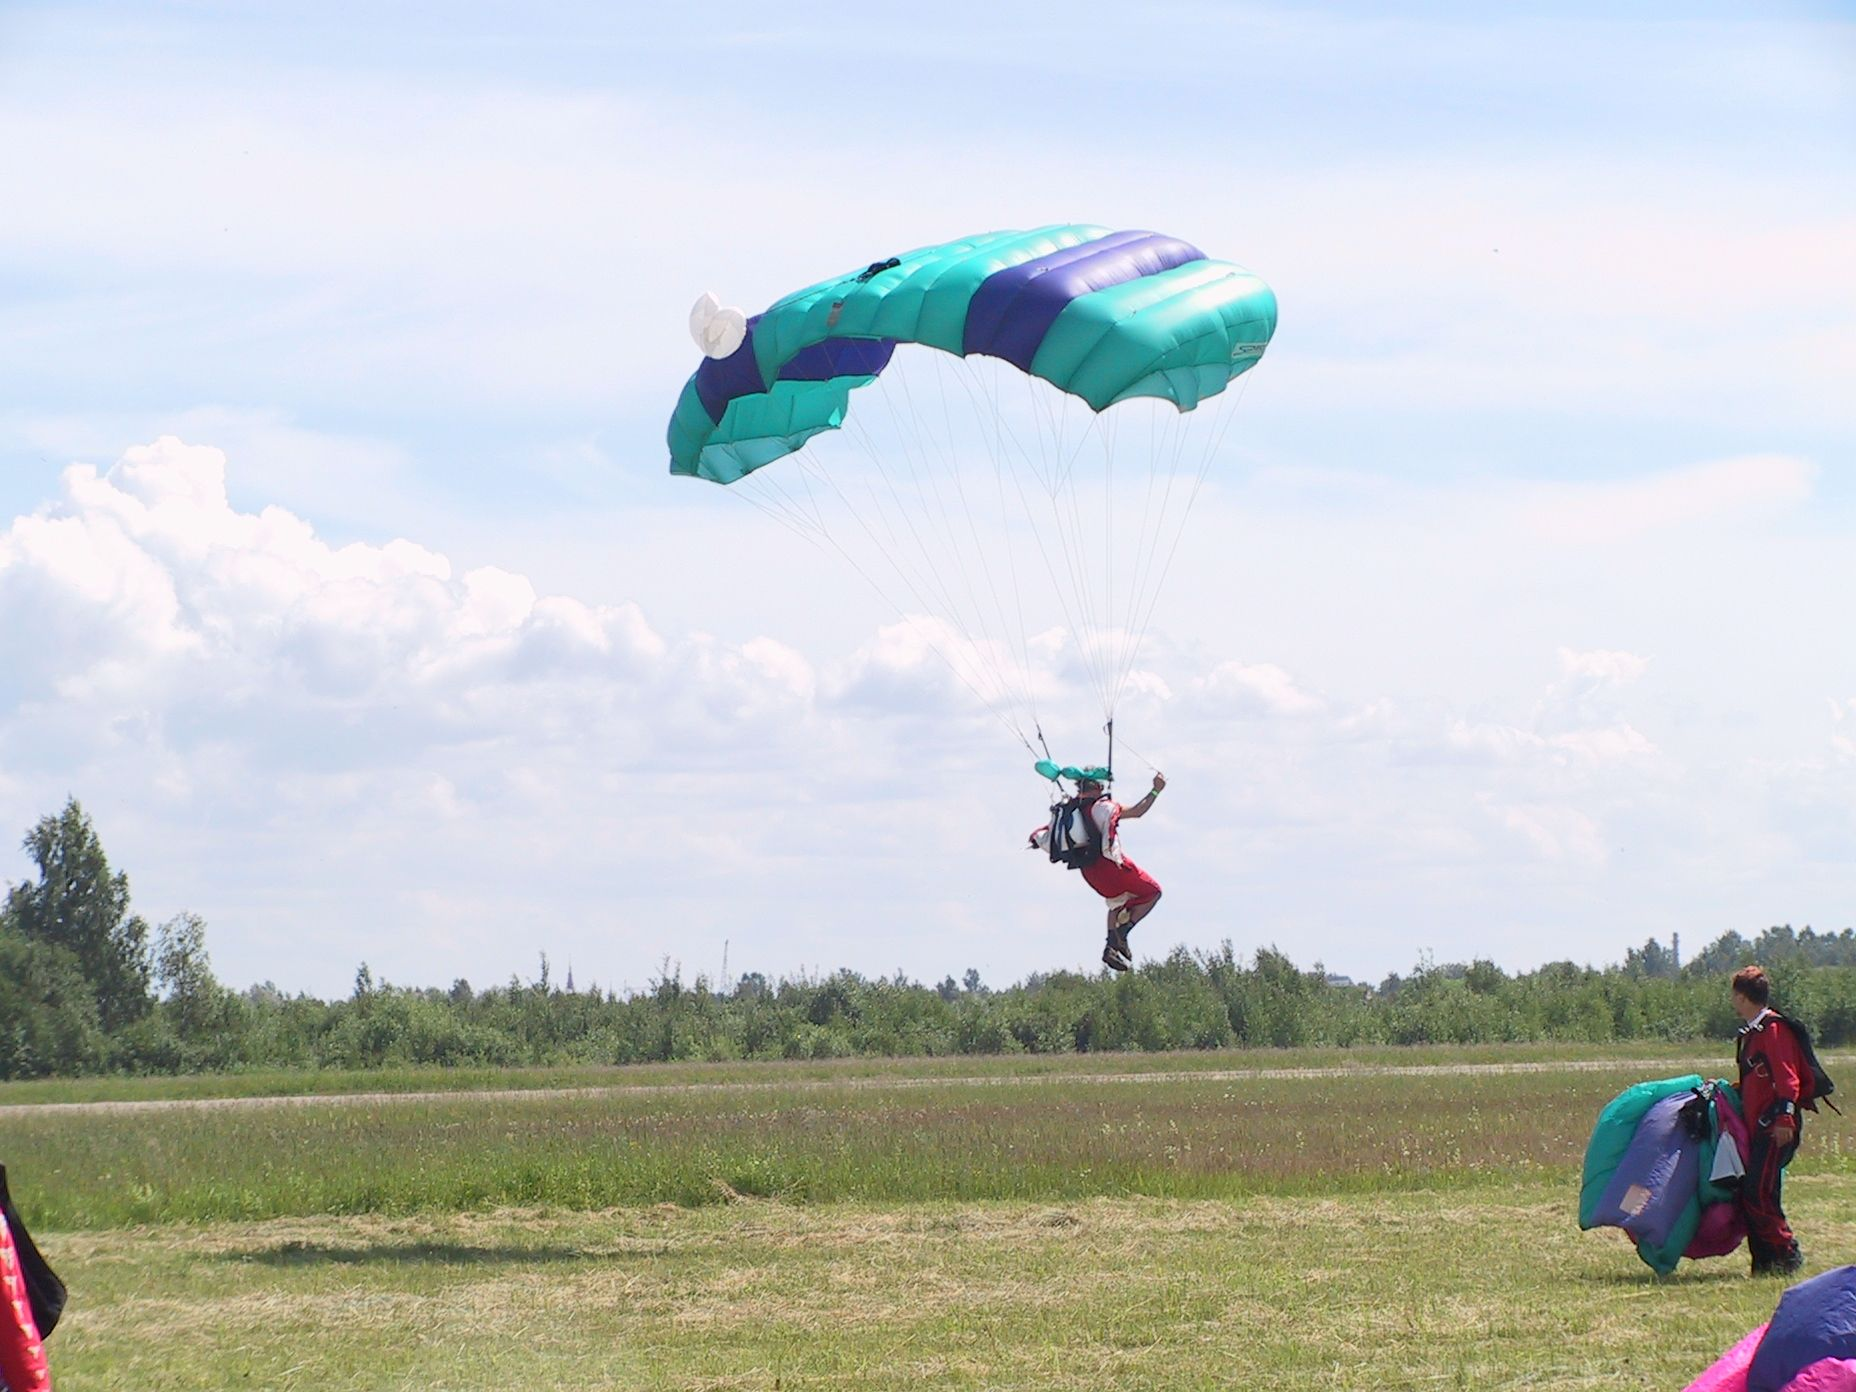
\includegraphics[width=0.99\textwidth]{Loppuveto_ylhaalla.jpeg}\captionof{figure}{Loppuveto liian ylhäällä ja kädet eri korkeuksilla.}\end{Figure}  

\section{ Loppuveto liian aikaisin tai liian myöhään }
\label{laskeutumisvirheet-loppuveto-liian-aikaisin-tai-liian-myohaan}


Jos loppuveto tehdään terävästi, mutta liian korkealla, jäädään \textit{hyllylle}. Se ei sinänsä ole suuri virhe, ellei lisäksi tehdä muita virheitä. Yleisimmät muut virheet ovat tasapainoansa ja sitä seuraava suojautumisansa, jolloin toinen jalka tai käsi pyrkii vastaanottamaan maakosketuksen ensimmäisenä. Tällöin valjaiden asento sekä varjon lentotila muuttuu ja varjo kääntyy. Ohjauslenkkien painaminen liian syvälle voi sakata varjon. Silloin on vaarana putoaminen maahan selälleen. Jos teet loppuvedon liian aikaisin, pidä kädet samalla tasolla ja varaudu kierähtämään. 


\begin{figure*}[]\centering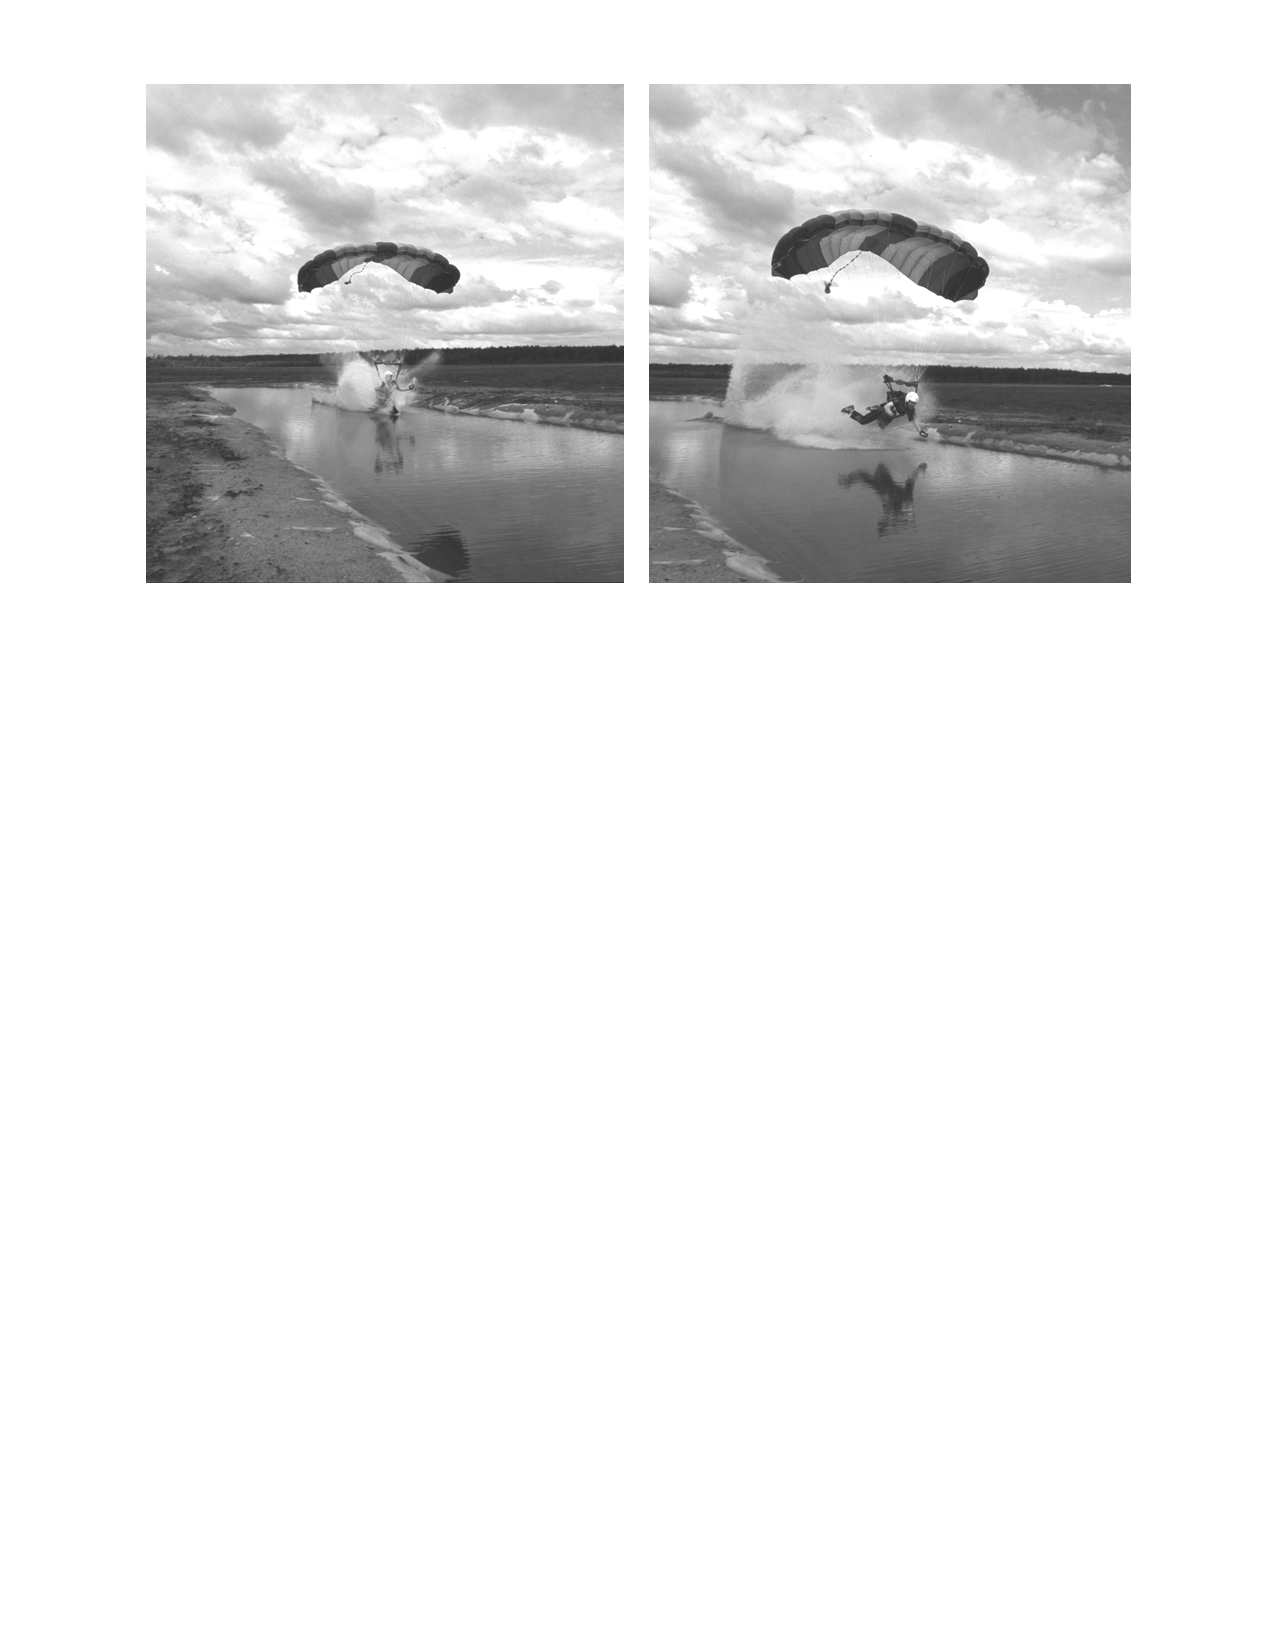
\includegraphics[width=0.9\textwidth]{Loppuveto-matala-pondi.pdf}\caption{Loppuveto liian myöhään, onneksi oli vettä pehmentämässä laskua.}\end{figure*}   


Liian myöhään tehty loppuveto ei ehdi kääntää varjon liikesuuntaa vaakalentoon, ja seurauksena on kova lasku. 

\section{ Liian pitkä tai voimakas loppuveto }
\label{laskeutumisvirheet-liian-pitka-tai-voimakas-loppuveto}


Liian pitkässä tai voimakkaassa loppuvedossa kuvun eteenpäin menevä vauhti loppuu hyppääjän jatkaessa matkaansa eteenpäin. Käsien ollessa alhaalla ja hyppääjän painopisteen siirtyminen eteenpäin aiheuttaa vaistomaisen refleksin suojata kaatumista käsillä. Pelivara on käytetty loppuun ja varjo sakkaa taakse. 


\begin{Figure}\centering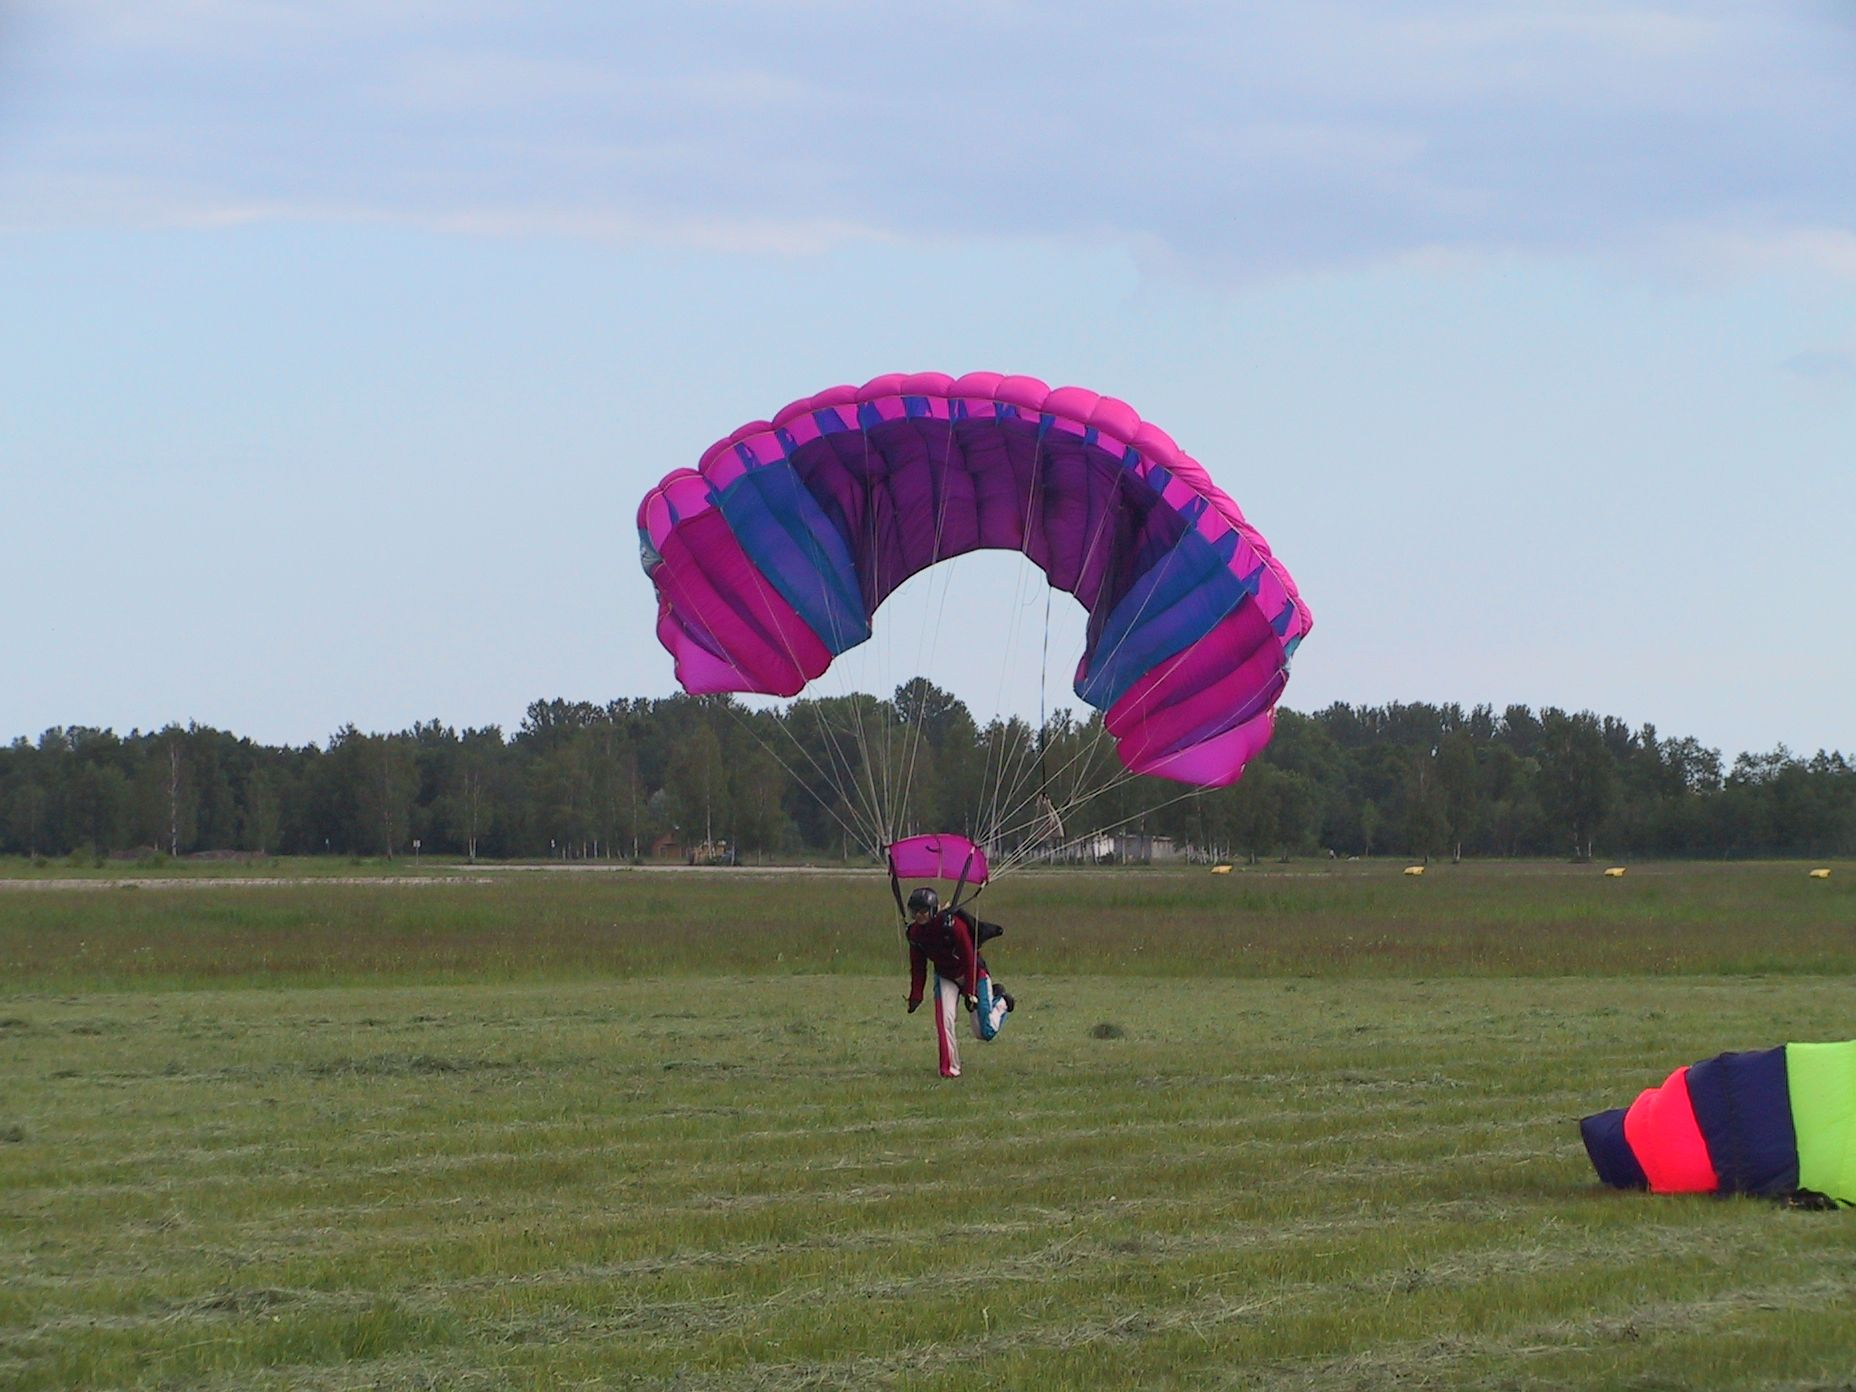
\includegraphics[width=0.99\textwidth]{Loppuveto-sakkaus.jpeg}\captionof{figure}{Hyppääjä on tehnyt loppuvedon liian pitkälle ja kupu sakkaa taakse hyppääjän jatkaessa vielä matkaa eteenpäin.}\end{Figure}  

\section{ Ei ohjata loppuun asti }
\label{laskeutumisvirheet-ei-ohjata-loppuun-asti}


Varjoa on ohjattava niin kauan kuin se lentää. Kun varjo on vaakalennossa, sillä on vielä paljon ilmanopeutta. Esimerkiksi yhden käden päästäminen irti ohjauslenkistä toisen käden vielä ollessa alhaalla kääntää kuvun vedon suuntaan. Lopeta ohjaaminen vasta vauhdin pysähdyttyä kokonaan. 

\section{ Suojautumisansa }
\label{laskeutumisvirheet-suojautumisansa}


\begin{figure*}[]\centering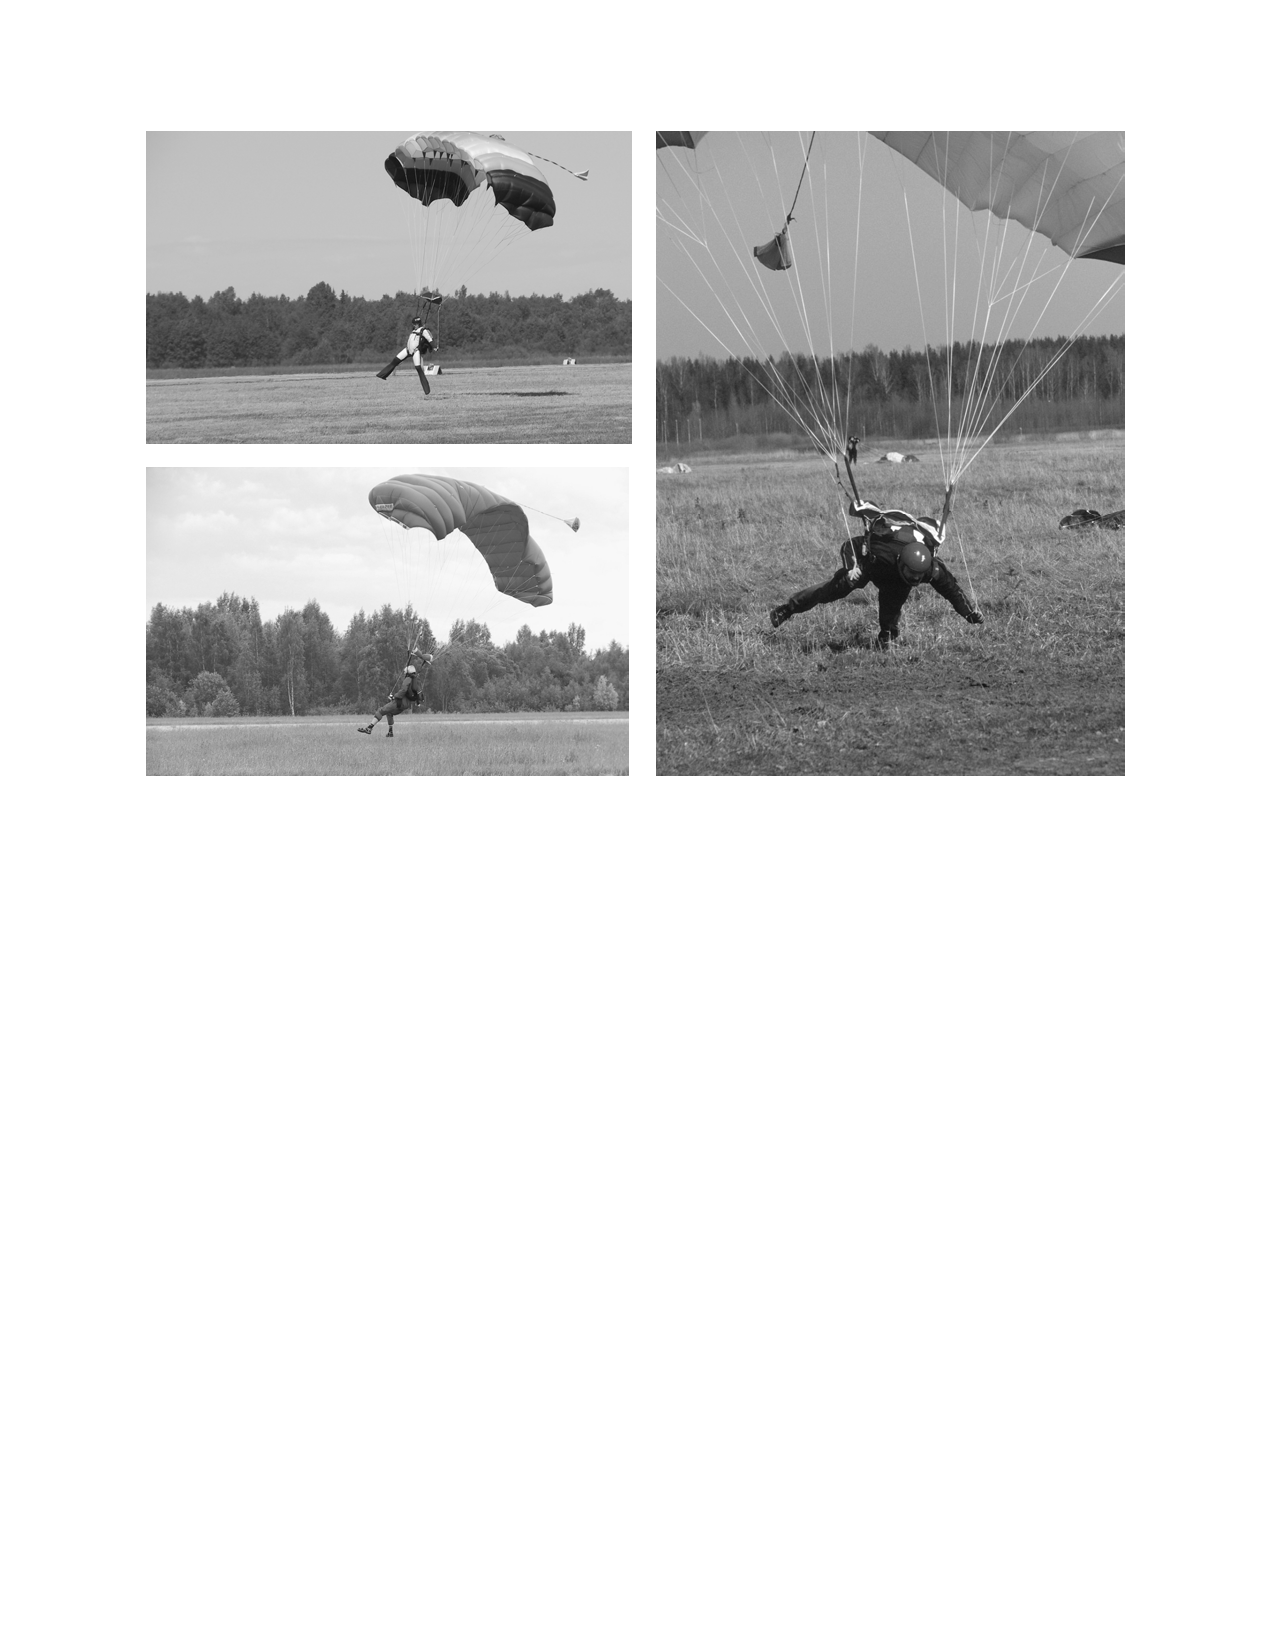
\includegraphics[width=0.9\textwidth]{Loppuveto-suojautumisansa.pdf}\caption{Suojautumisansa - hyppääjä kurottaa kädellään ja jalallaan maata, varjo kaatuu kurottamisen suuntaan.}\end{figure*} 


Suojautumisansassa hyppääjä suojaa vaistomaisesti kaatumista käsillään tai jaloillaan. Kun ohjauslenkit ovat käsissä ja painopiste siirtyy, liike vaikuttaa suoraan kupuun ja lisää varjon kääntymistä/jarrutusta. Jalalla suojauduttaessa valjaiden asento muuttuu ja vaikutus on edellä kuvatun kaltainen. Suojautumisansa on ihmiselle luontainen refleksi. 

\section{ Tasapainoansa }
\label{laskeutumisvirheet-tasapainoansa}


Tasapainoansassa hyppääjän tasapaino horjuu ja hyppääjä tuntee olevansa kuin nuorallatanssija. Hän kompensoi sivulle kaatumista nostamalla vastakkaisen puolen kättä ylös. Tällöin varjo kääntyy yhä jyrkemmin, ja seuraa suojautumisansa. Tämä korostuu esimerkiksi skysurf-laudalla hypätessä, jolloin alavartaloa ei voi käyttää tasapainon pitämiseen. Tasapainoansa on ihmisen luontainen refleksi. 


\begin{Figure}\centering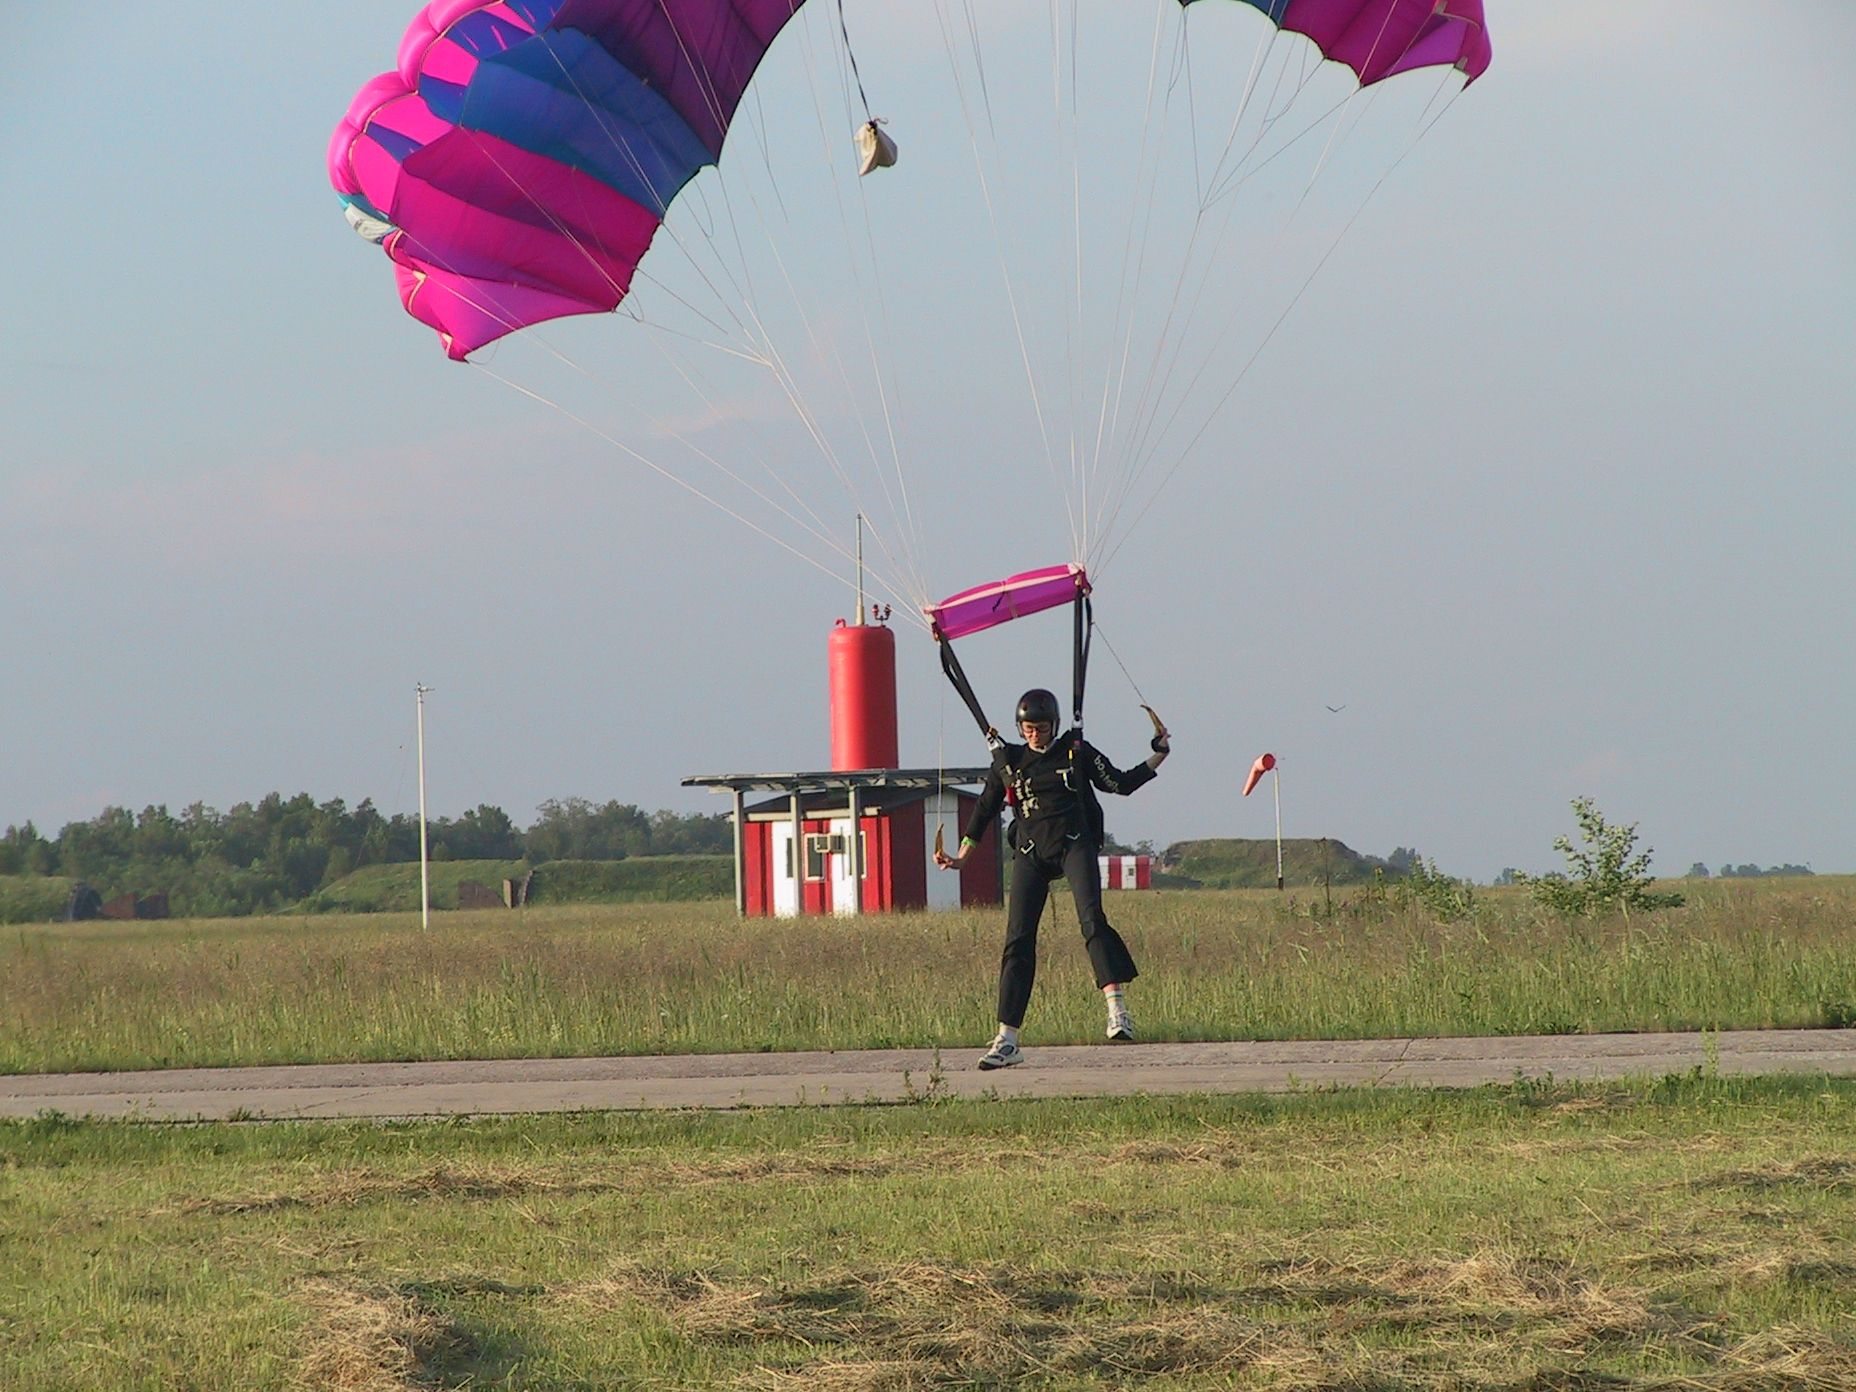
\includegraphics[width=0.7\textwidth]{Tasapainoansa.jpeg}\captionof{figure}{Tasapainoansa. Hyppääjä on nostanut vasemman kätensä ja samalla kurkottaa oikealla jalallaan maata (suojautumisansa), varjo kaatuu oikealle.}\end{Figure}  

\section{ Kädet nousevat ylös jalkojen koskettaessa maata }
\label{laskeutumisvirheet-kadet-nousevat-ylos-jalkojen-koskettaessa-maata}


Ihmisellä on useita vaistomaisia refleksejä, jotka tapahtuvat nopeasti ja huomataan vasta videolta katsottaessa. Joillakin hyppääjillä kädet nousevat hetkellisesti ylös, kun jalat koskettavat maata. Tästä seuraa kuvun hyökkääminen eteenpäin ja sen seurauksena painopisteen siirtyminen taaksepäin ja kaatuminen. Keskity kuvun ohjaamiseen nostamatta käsiä. 

\section{ Kädet liikkuvat juostessa }
\label{laskeutumisvirheet-kadet-liikkuvat-juostessa}


Loppuvedon jälkeen vaakalennossa, vauhdin ollessa vielä suuri ja jouduttaessa juoksemaan vauhti pois, on syytä juosta siten, että kädet pysyvät mahdollisimman liikkumatta. Käsien heiluttaminen juoksun tahdissa vaikuttaa suoraan varjon lentämiseen ja seurauksena voi olla varjon kaatuminen sivulle. 


\begin{Figure}\centering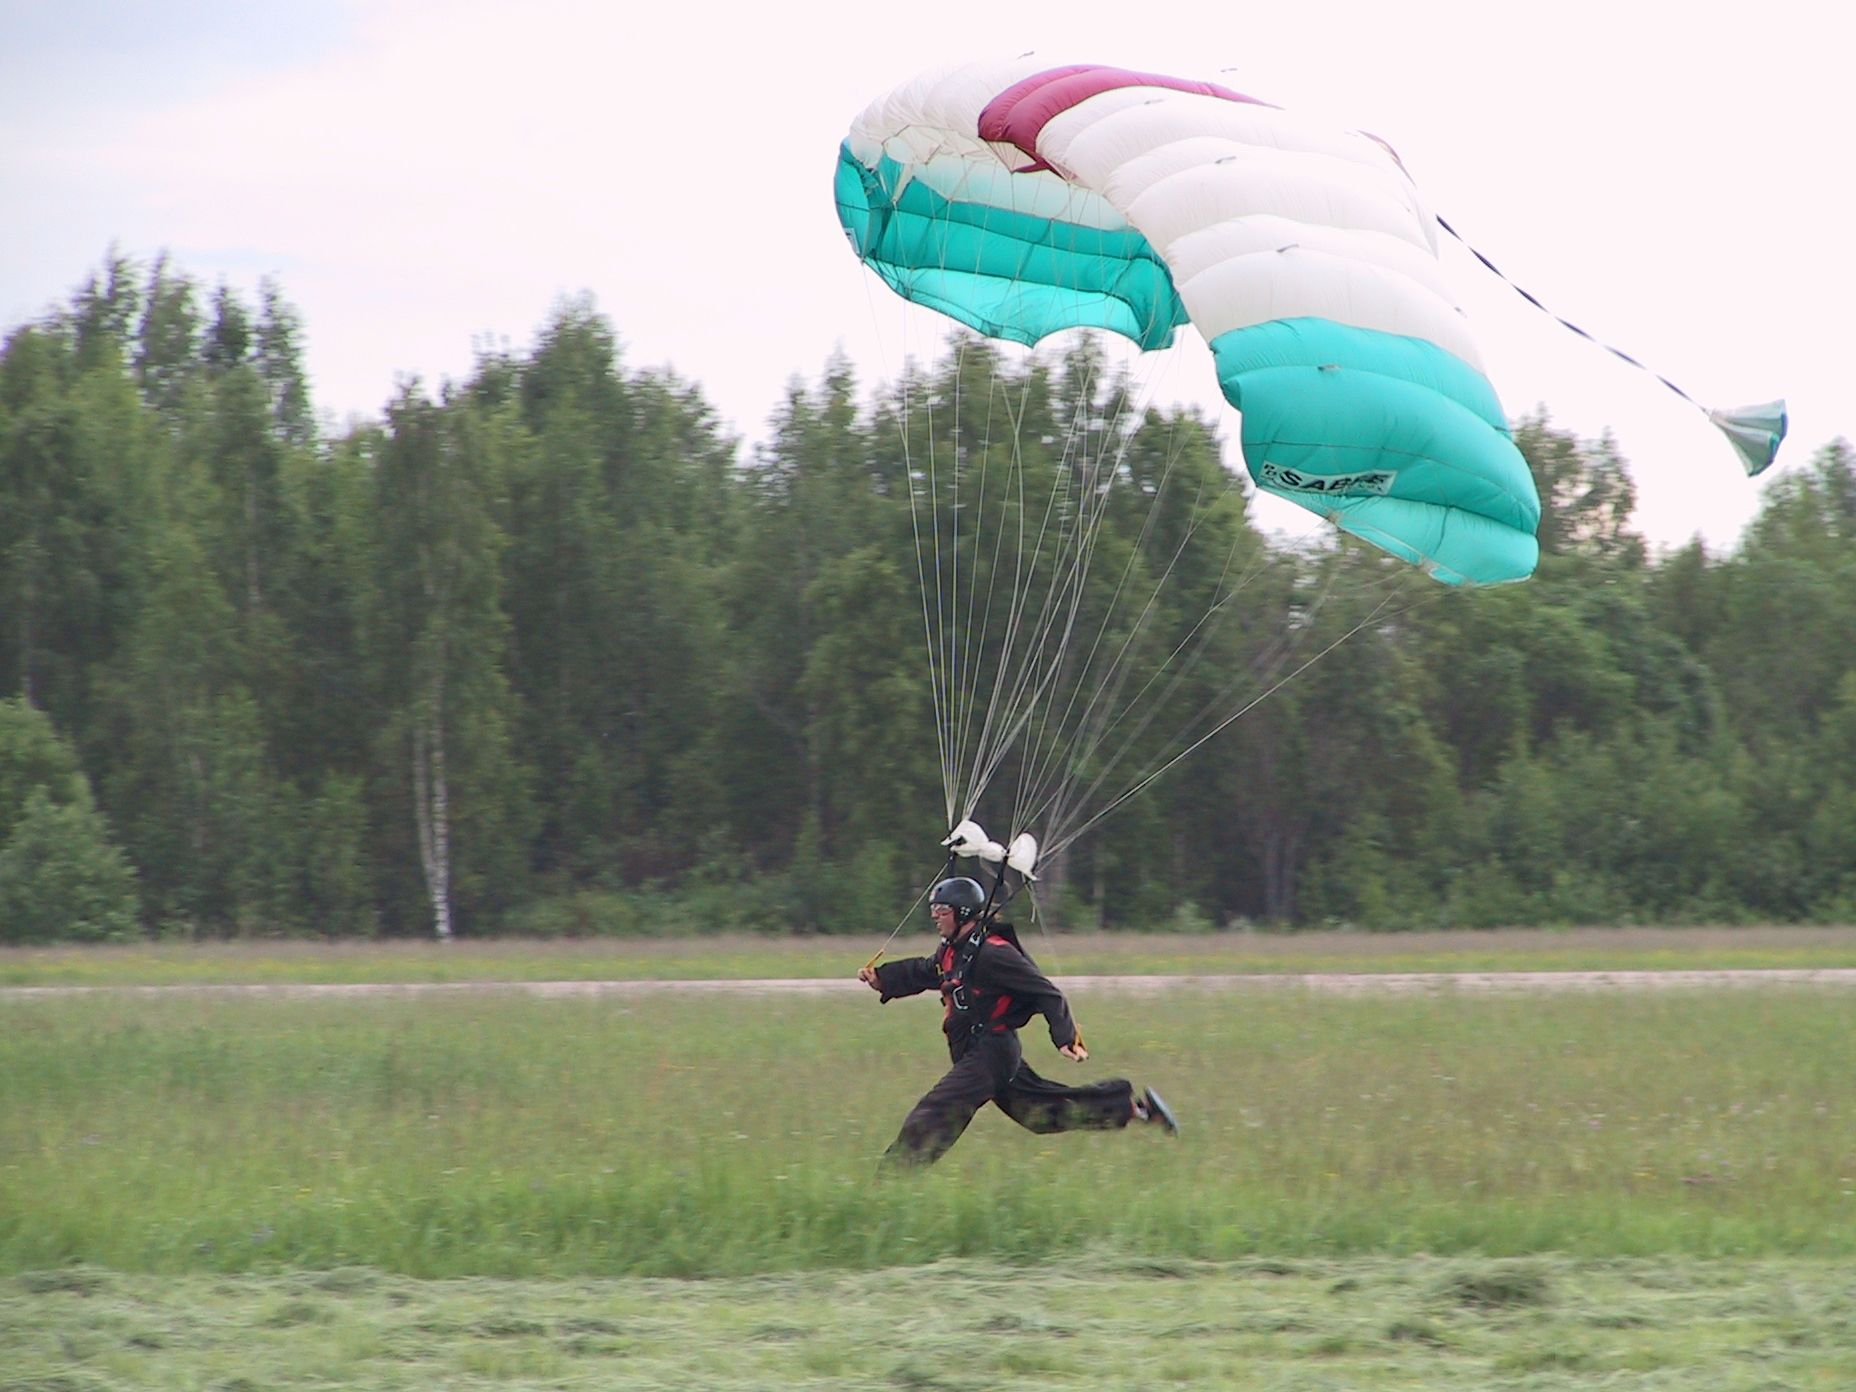
\includegraphics[width=0.7\textwidth]{Laskeutuminen_kadet_liikkuvat.jpeg}\captionof{figure}{Kädet eivät pysy samalla tasolla juostessa ja kupu kaatuu vasemmalle.}\end{Figure} 

\section{ Jalat nousevat ylös loppuvedossa }
\label{laskeutumisvirheet-jalat-nousevat-ylos-loppuvedossa}


Yksi vaistomaisista reflekseistä on jalkojen nostaminen, kun kädet vetävät loppuvedon. Seurauksena on laskeutuminen istualleen. Keskity kuvun ohjaamiseen nostamatta jalkoja. Kovassa laskussa takamukselle selkäranka voi saada vaurioita. 


\begin{Figure}\centering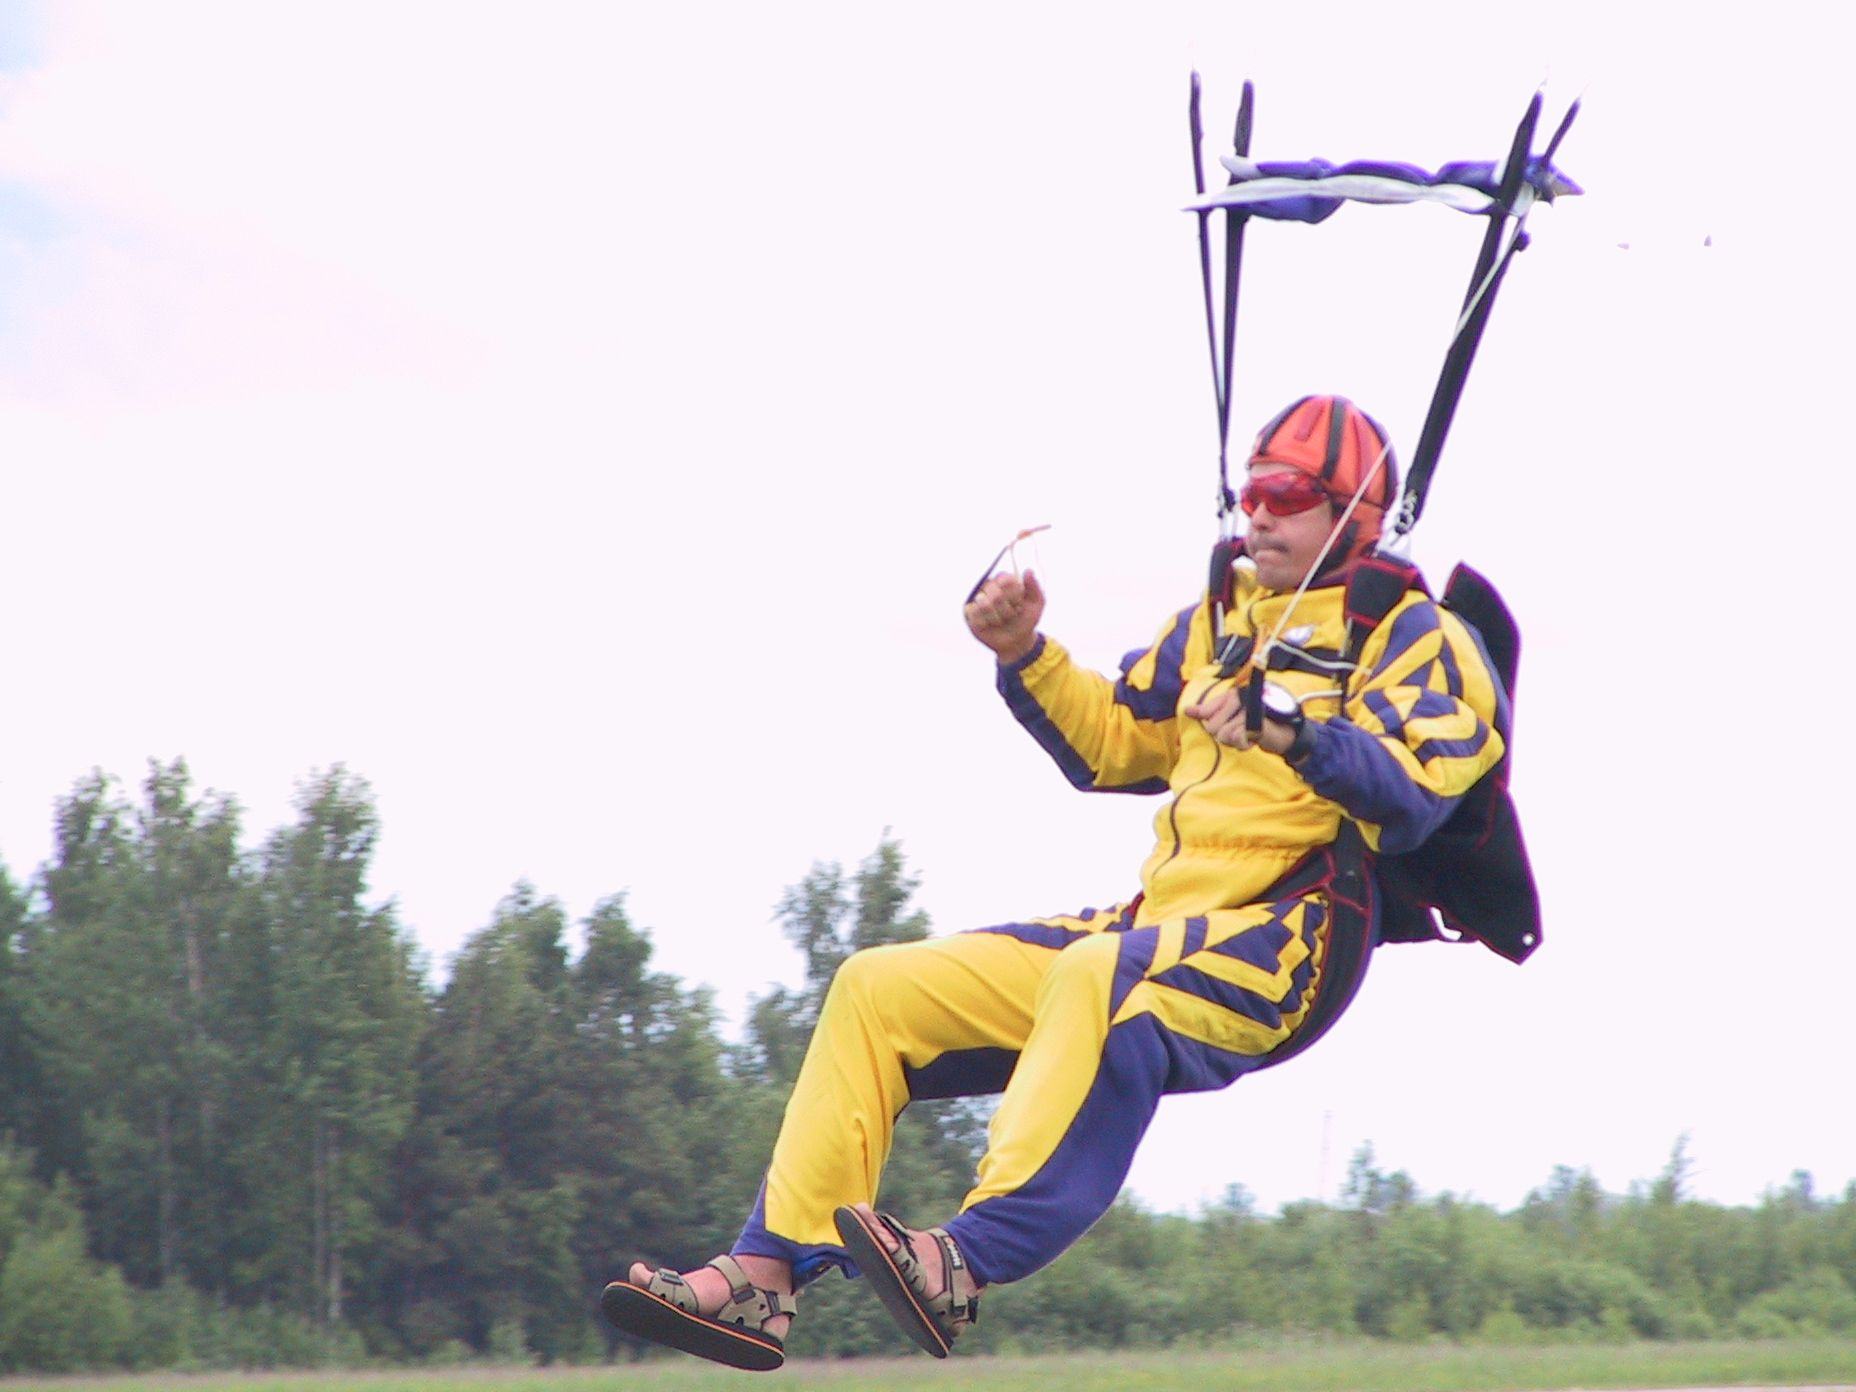
\includegraphics[width=0.7\textwidth]{Laskeutuminen_jalat_ylos.jpeg}\captionof{figure}{Hyppääjä tekee loppuvedon nostaen samalla jalat ylös eteen.}\end{Figure} 

